\documentclass[12pt]{amsart}
\pdfoutput=1
\usepackage{latexsym, amsmath, amssymb, amsthm, bm}
\usepackage{calrsfs}
\usepackage{subfig}

\usepackage[mathscr]{eucal}
\usepackage{mathtools}
\usepackage{paralist}
\usepackage[alphabetic]{amsrefs}
\usepackage[T1]{fontenc}
\usepackage{mathptmx}
\usepackage{microtype}
\usepackage{tikz}
\renewcommand{\baselinestretch}{1.05}
\usepackage[colorlinks=true,linkcolor=blue,urlcolor=blue, citecolor=blue]%
    {hyperref}
\linespread{1.06}
%%--LAYOUT--------------------------------------------------------------------
\usepackage[paperwidth=8.5in, paperheight=11in, inner=2.5cm, outer=2.5cm,% 
    top=2.5cm, bottom=2.5cm]{geometry}
%%--OTHER ENVIRONMENTS--------------------------------------------------------
\newtheorem{lemma}{Lemma}[section]
\newtheorem{theorem}[lemma]{Teorema}
\newtheorem{corollary}[lemma]{Corolario}
\newtheorem{proposition}[lemma]{Proposición}
\theoremstyle{definition}
\newtheorem{definition}[lemma]{Definición}
\newtheorem{remark}[lemma]{Observación}
\newtheorem{examplex}[lemma]{Ejemplo}
\newtheorem{procedure}[lemma]{Procedure}

\newenvironment{exm}
  {\pushQED{\qed}\renewcommand{\qedsymbol}{$\diamond$}\examplex}
  {\popQED\endexamplex}
\newtheorem{question}[lemma]{Question}
\newtheorem{conjecture}[lemma]{Conjecture}
\newtheorem{Construction}[lemma]{Construction}
\newtheorem{algorithm}[lemma]{Algorithm}
%\theoremstyle{remark}
\newcommand{\define}[1]{{\bfseries\itshape #1}}
%%--MATH----------------------------------------------------------------------
\newcommand{\relphantom}[1]{\mathrel{\phantom{#1}}}
\newcommand{\abs}[1]{\ensuremath{\left| #1 \right|}}
%\newcommand{\norm}[1]{\ensuremath{\left\| #1 \right\|}}
\newcommand{\ideal}[1]{\ensuremath{\left\langle #1 \right\rangle}}
\renewcommand{\geq}{\geqslant}
\renewcommand{\leq}{\leqslant}
\newcommand{\coloneq}{\ensuremath{\mathrel{\mathop :}=}}
\newcommand{\transpose}{\ensuremath{\textsf{\upshape T}}} 
%% Blackboard bolds symbols
\renewcommand{\AA}{\ensuremath{\mathbb{A}}} 
\newcommand{\CC}{\ensuremath{\mathbb{C}}} 
\newcommand{\kk}{\ensuremath{\Bbbk}} 
\newcommand{\NN}{\ensuremath{\mathbb{N}}}
\newcommand{\PP}{\ensuremath{\mathbb{P}}} 
\newcommand{\QQ}{\ensuremath{\mathbb{Q}}} 
\newcommand{\RR}{\ensuremath{\mathbb{R}}} 
\newcommand{\EE}{\ensuremath{\mathbb{E}}} 

\renewcommand{\P}{\ensuremath{P}} 
\newcommand{\Q}{\ensuremath{Q}} 

%\renewcommand{\SS}{\ensuremath{\mathbb{S}}} 
\newcommand{\ZZ}{\ensuremath{\mathbb{Z}}} 
%% Script symbols
\newcommand{\sC}{\ensuremath{\mathcal{C}}}
\newcommand{\sE}{\ensuremath{\mathcal{E}}}
\newcommand{\sF}{\ensuremath{\mathcal{F}}}
\newcommand{\calF}{\ensuremath{\mathcal{F}}}
\newcommand{\calL}{\ensuremath{\mathcal{L}}}

\newcommand{\sH}{\ensuremath{\mathcal{H}}}
\newcommand{\sL}{\ensuremath{\mathcal{L}}}
\newcommand{\sO}{\ensuremath{\mathcal{O}}}

\newcommand{\diam}{\operatorname{diam}}
\newcommand{\Osh}{{\mathcal O}}
\newcommand{\Ish}{{\mathcal I}}
\newcommand{\calI}{{\mathcal I}}

%% Operators
\DeclareMathOperator{\codim}{codim}
\DeclareMathOperator{\coker}{Coker}
\DeclareMathOperator{\conv}{conv}
\DeclareMathOperator{\Cox}{Cox}
\DeclareMathOperator{\depth}{depth}
\DeclareMathOperator{\gon}{gon}
\DeclareMathOperator{\Grass}{Gr}
\DeclareMathOperator{\green}{\textit{a}}
\DeclareMathOperator{\HH}{H}
\DeclareMathOperator{\HHH}{\mathbb{H}}
\DeclareMathOperator{\Hom}{Hom}
\DeclareMathOperator{\id}{id}
\DeclareMathOperator{\Image}{Im}
\DeclareMathOperator{\kept}{\lambda}
\DeclareMathOperator{\Ker}{Ker}
\DeclareMathOperator{\len}{\ell}
\DeclareMathOperator{\py}{py}
\DeclareMathOperator{\Pic}{Pic}
\DeclareMathOperator{\Proj}{Proj}
\DeclareMathOperator{\pr}{p}
\DeclareMathOperator{\qp}{qp}
\DeclareMathOperator{\qr}{qr}
\DeclareMathOperator{\rank}{rank}
\DeclareMathOperator{\reg}{reg}
\DeclareMathOperator{\Sos}{\Sigma}
\DeclareMathOperator{\Span}{Span}
\DeclareMathOperator{\Spec}{Spec}
\DeclareMathOperator{\sw}{sw}
\DeclareMathOperator{\Sym}{Sym}
\DeclareMathOperator{\topint}{int}
\DeclareMathOperator{\Tor}{Tor}
\DeclareMathOperator{\tw}{tw}
\DeclareMathOperator{\variety}{V}
%% Personalized comments
\newcommand\mv[1]{{\color{blue}(MV: #1)}}
\newcommand\mve[1]{{\color{red}(MV: #1)}}
\newcommand\jh[1]{{\color{red}(JH: #1)}}

\title{Guía de estudio I (Probabilidad y Estadística)}

\begin{document}
\maketitle
El objetivo de este documento es servir de guía para les estudiantes en su preparación para los parciales del curso.
Los enunciados marcados con Lema o Teorema son fundamentales y hay que conocer sus demostraciones.


\section{Definiciones básicas}

{\bf Notación.} Usaremos los conceptos de unión, intersección e inclusión de conjuntos. Para dos conjuntos $A,B$ escribiremos $AB:=A\cap B$ para simplificar las fórmulas.



\begin{definition} Un \emph{espacio de probabilidad} es una tripla $(\Omega,\calF,\PP)$ donde:

\begin{enumerate}
\item $\Omega$ es un conjunto cualquiera, llamado \emph{espacio muestral}
\item $\calF$ es una \emph{sigma-algebra} de subconjuntos de $\Omega$, es decir una colección de subconjuntos que cumple las siguientes condiciones:
\begin{enumerate}
\item (\emph{No vacuidad}) $\Omega\in \calF$
\item (\emph{Cerradura bajo complementos}) $A\in \calF$ entonces $\overline{A}\in \calF$ donde $\overline{A}:=\Omega\setminus A$.
\item (\emph{Cerradura bajo uniones contables}) Si $\{A_n\}_{n\in \mathbb{N}}$ es una colección de conjuntos con $A_j\in \calF$ entonces $\bigcup_{n\in \mathbb{N}} A_j\in \calF$.
\end{enumerate}
\item $\PP$ es una \emph{medida de probabilidad}, es decir una funci\'on $\PP: \calF\rightarrow \RR$ que cumple:
\begin{enumerate}
\item (\emph{no-nonegatividad}) $\forall A\in \calF\left(\PP(A)\geq 0\right)$
\item (\emph{máximo uno}) $\PP(\Omega)=1$
\item (\emph{es $\sigma$-aditiva sobre conjuntos disjuntos}) Si $A_j$, $j=1,2,3,\dots$ es una colección de conjuntos disjuntos (i.e. si $A_i\cap A_j=\emptyset$ para $i\neq j$) con $A_j\in \calF$ entonces 
\[\PP\left(\bigcup_{j=0}^\infty A_j\right)=\sum_{j=0}^{\infty} \PP(A_j)\]
\end{enumerate} 
\end{enumerate}
\end{definition}

Los axiomas de arriba permiten deducir propiedades que se cumplen en todos los espacios de probabilidad. El siguiente Lema contiene algunas de esas propiedades (intente demostrarlas para verificar su entendimiento de los axiomas básicos)

\begin{lemma} Sea $(\Omega,\calF,\PP)$ un espacio de probabilidad. Demuestre que las siguientes propiedades se cumplen:

\begin{enumerate}
\item Para todo $A\in \calF$ se tiene $\PP(\overline{A})=1-\PP(A)$
\item Si $A,B\in \calF$ con $A\subseteq B$ entonces $\PP(A)\leq \PP(B)$. En particular la probabilidad de cualquier evento $A\in\calF$ cumple $\PP(A)\leq 1$.
\item Para todos $A,B\in \calF$ se tiene que 
\[\PP(A\cup B)=\PP(A)+\PP(B)-\PP(A\cap B).\]
Más generalmente si $A,B,C$ son tres eventos cualquiera se tiene que
\[\PP(A\cup B\cup C)=\PP(A)+\PP(B)+\PP(C)-\left(\PP(AB)+\PP(AC)+\PP(BC)\right)+\PP(ABC)\]
\item (\emph{Union bound}) Si $A_1,A_2,\dots\in\calF$ son una colección cualquiera de eventos, entonces \[\PP\left(\bigcup_{j=1}^\infty A_j\right)\leq \sum_{j=1}^\infty \PP(A_j).\]
\end{enumerate}
\end{lemma}


\subsection{Ejemplo 1: La probabilidad clásica ó la medida Uniforme sobre conjuntos finitos}

Si $\Omega$ es un conjunto finito cualquiera definimos $\calF$ como la coleccion de todos los subconjuntos de $\Omega$ y $\PP(A):=\frac{|A|}{|\Omega|}$ para cualquier subconjunto $A\subseteq \Omega$. Es fácil verificar que $(\Omega,\calF,\PP)$ es un espacio de probabilidad llamado \emph{probabilidad uniforme en $\Omega$}.
Por definición la probabilidad uniforme se calcula contando cuántos casos favorables hay $|A|$ y dividiéndolo sobre el número de casos totales $|\Omega|$. La rama de las matemáticas que se ocupa de contar se llama combinatoria. Para poder resolver problemas de conteo necesitamos algunos fundamentos de combinatoria que resumimos a continuación en las

{\bf Reglas de conteo:}
\begin{enumerate}
\item (\emph{principio del producto}) Si un proceso se realiza en $n$ etapas y hay $a_1$ maneras para realizar la primera etapa, $a_2$ maneras de realizar la segunda (independientemente de la primera elección), $a_3$ maneras de realizar la tercera (independientemente de las primeras dos elecciones), etc. entonces el número total de maneras de realizar el proceso es el producto
\[a_1\cdot a_2\cdot\dots \cdot a_n\] 
\item (\emph{principio de la suma}) Si $A,B$ son conjuntos disjuntos entonces 
\[|A\cup B|=|A|+|B|\]
\end{enumerate}
\noindent 
El siguiente Lema contiene algunas propiedades básicas de combinatoria que usaremos de ahora en adelante. Demuéstrelo para verificar su entendimiento de los principios

\begin{lemma} Las siguientes afirmaciones son ciertas:
\begin{enumerate}
\item El número de palabras de longitud $n$ en los símbolos $1,2,\dots,k$ es $k^n$.
\item El número de palabras de longitud $n$ en los símbolos $1,2,\dots,k$ en las que cada símbolo se usa a lo más una vez es
\[k(k-1)(k-2)\dots (k-n+1)=\frac{k!}{(k-n)!}\]

\item El número de subconjuntos de tamaño $k$ de un conjunto de $n$ items, denotado $\binom{n}{k}$ esta dado por
\[\binom{n}{k}=\frac{n!}{k!(n-k)!}\]
\end{enumerate}

\end{lemma}


\begin{examplex}
Una baraja consiste de $52$ cartas. Cada carta tiene una pinta (diamantes, corazones, picas o tréboles) y en cada pinta tiene uno de trece símbolos
$1,2,\dots,10,J,Q,K$ (el uno también se llama As). Hay pintas de dos colores, rojas y negras: diamantes y corazones son rojas y las demás negras.

En el juego del Poker se reparten \emph{uniformemente} $5$ cartas a cada jugador. Calcule las probabilidades de que un jugador tenga cada una de las siguientes manos:

\begin{enumerate}
    \item \emph{Un par}: exactamente dos cartas tienen el mismo símbolo y las otras tres cartas tienen símbolos distintos entre sí y distintos del símbolo del par.

    \item \emph{Dos pares}: hay dos pares de cartas con el mismo símbolo, y la quinta carta tiene un símbolo distinto de los otros cuatro.

    \item \emph{Trío}: exactamente tres cartas tienen el mismo símbolo y las otras dos cartas tienen símbolos distintos entre sí y distintos del símbolo del trío.

    \item \emph{Escalera}: las cinco cartas tienen símbolos consecutivos, independientemente de sus pintas. En este caso, el As puede utilizarse como $1$ en la secuencia
    $A,2,3,4,5$ o como la carta inmediatamente superior al Rey en
    $10,J,Q,K,A$.

    \item \emph{Color}: las cinco cartas tienen la misma pinta, pero no forman una escalera.

    \item \emph{Full}: tres cartas tienen el mismo símbolo y las otras dos cartas tienen otro símbolo en común.

    \item \emph{Póker}: cuatro cartas tienen el mismo símbolo y la quinta carta tiene un símbolo diferente.

    \item \emph{Escalera de color}: las cinco cartas tienen la misma pinta y sus símbolos son consecutivos. Incluye la escalera real
    $10,J,Q,K,A$.
\end{enumerate}
\end{examplex}

\subsection{Ejemplo 2: Intentos de Bernoulli}

Los Bernoulli trials son un modelo probabilista para la siguiente situación: \emph{Se lanzan $n$ monedas independientemente. Cada una de las monedas tiene dos lados (llamados $0$ y $1$). Sabemos que la probabilidad de que cada moneda salga $1$ es un número conocido $p\in [0,1]$.}


Para poder formalizar el concepto de independencia debemos entender cómo debe alterarse la probabilidad cuando sabemos que un evento $B$ ha ocurrido. Esto esta capturado por la probabilidad condicional $\PP(A|B)$.

\begin{definition} Si $B\in \calF$ es un evento con $\PP(B)>0$ definimos, para cualquier $A\in \calF$ la \emph{probabilidad condicional de $A$ dado $B$} mediante la fórmula
\[\PP\left(A|B\right)=\frac{\PP\left(A\cap B\right)}{\PP\left(B\right)}\]
\end{definition}

Dos eventos $A$ y $B$ son $\PP$- independientes si saber que $B$ ocurrió no afecta la probabilidad de que $A$ ocurra, es decir
\[\PP(A|B)=\PP(A)\] 
Usando la definición de probabilidad condicional esto es equivalente a
\[\PP(A\cap B)=\PP(A)\PP(B)\] 
Generalizando lo anterior definimos

\begin{definition} Un conjunto de eventos $A_1,\dots, A_n$ se dicen \emph{eventos $\PP$-independientes} si para cualquier subconjunto de índices $I\subseteq \{1,\dots, n\}$ tenemos la igualdad
\[\PP\left(\bigcap_{j\in I} A_j\right)=\prod_{j\in I} \PP(A_j)\]
\end{definition}
\begin{remark} En la literatura en probabilidades típicamente se escribe \emph{independientes} en lugar de $\PP$-independientes. No obstante la independencia no solo depende de los eventos $A,B$ sino tambien de la medida de probabilidad que estemos usando.
\end{remark}

\begin{examplex} (\emph{Bernoulli trials}) Se lanzan $n$ monedas independientemente. Cada una de las monedas tiene dos lados (llamados $0$ y $1$). Sabemos que la probabilidad de que cada moneda salga $1$ es un número conocido $p\in [0,1]$.\\

Denotamos $q:=1-p$. Describiremos un modelo probabilístico para los Bernoulli trials. Definimos $\Omega=\{0,1\}^n$ como el conjunto de palabras de longitud $n$ en el conjunto de símbolos $\{0,1\}$ Una palabra $\omega\in \Omega$ describe completamente el resultado de los $n$ lanzamientos. Si $n=3$ la palabra $\omega=(1,1,0)$ dice que la primera y segunda moneda salieron $1$ y la tercera cero. Definimos $\calF$ como todos los subconjuntos de $\Omega$.
Para una palabra $\omega\in \Omega$ definimos
\[\PP(\{\omega\})=p^{n_1(\omega)}q^{n_0(\omega)}\]
donde $n_0(\omega)$ es el número de ceros en la palabra $\omega$ y $n_1(\omega)$ es el número de unos.
Para los demás $A\in \calF$ definimos $\PP(A):=\sum_{\omega\in A}\PP(\omega)$.
\end{examplex}

El siguiente Lema contiene las propiedades principales del modelo de Bernoulli.

\begin{lemma}Para $j=1,\dots, n$ defina 
$C_j:=\{\omega\in \Omega: \omega_j=1\}.$
Las siguientes propiedades se cumplen en el $(\Omega,\calF, \PP)$ definido anteriormente
\begin{enumerate}
\item $\PP(C_j)=p$
\item Los conjuntos $C_j$ son eventos $\PP$-independientes.
\end{enumerate}
Más aún, existe una única medida de probabilidad $\PP$ en $(\Omega, \calF)$ que satisface estas dos propiedades.
\end{lemma}

Teniendo una medida de probabilidad podemos calcular como se comporta cualquier cantidad que queramos medir sobre los $n$ lanzamientos. Por ejemplo,


\begin{lemma} (\emph{Distribución binomial}) Sea $S:\Omega\rightarrow \RR$ el número de éxitos (cantidad de $1$'s) en los $n$ lanzamientos. Para $k=0,\dots, n$ se tiene que
\[\PP\{\omega\in \Omega: S(\omega)=k\}:=\binom{n}{k}p^kq^{n-k}\]
\end{lemma}

\begin{figure}[h]
\centering
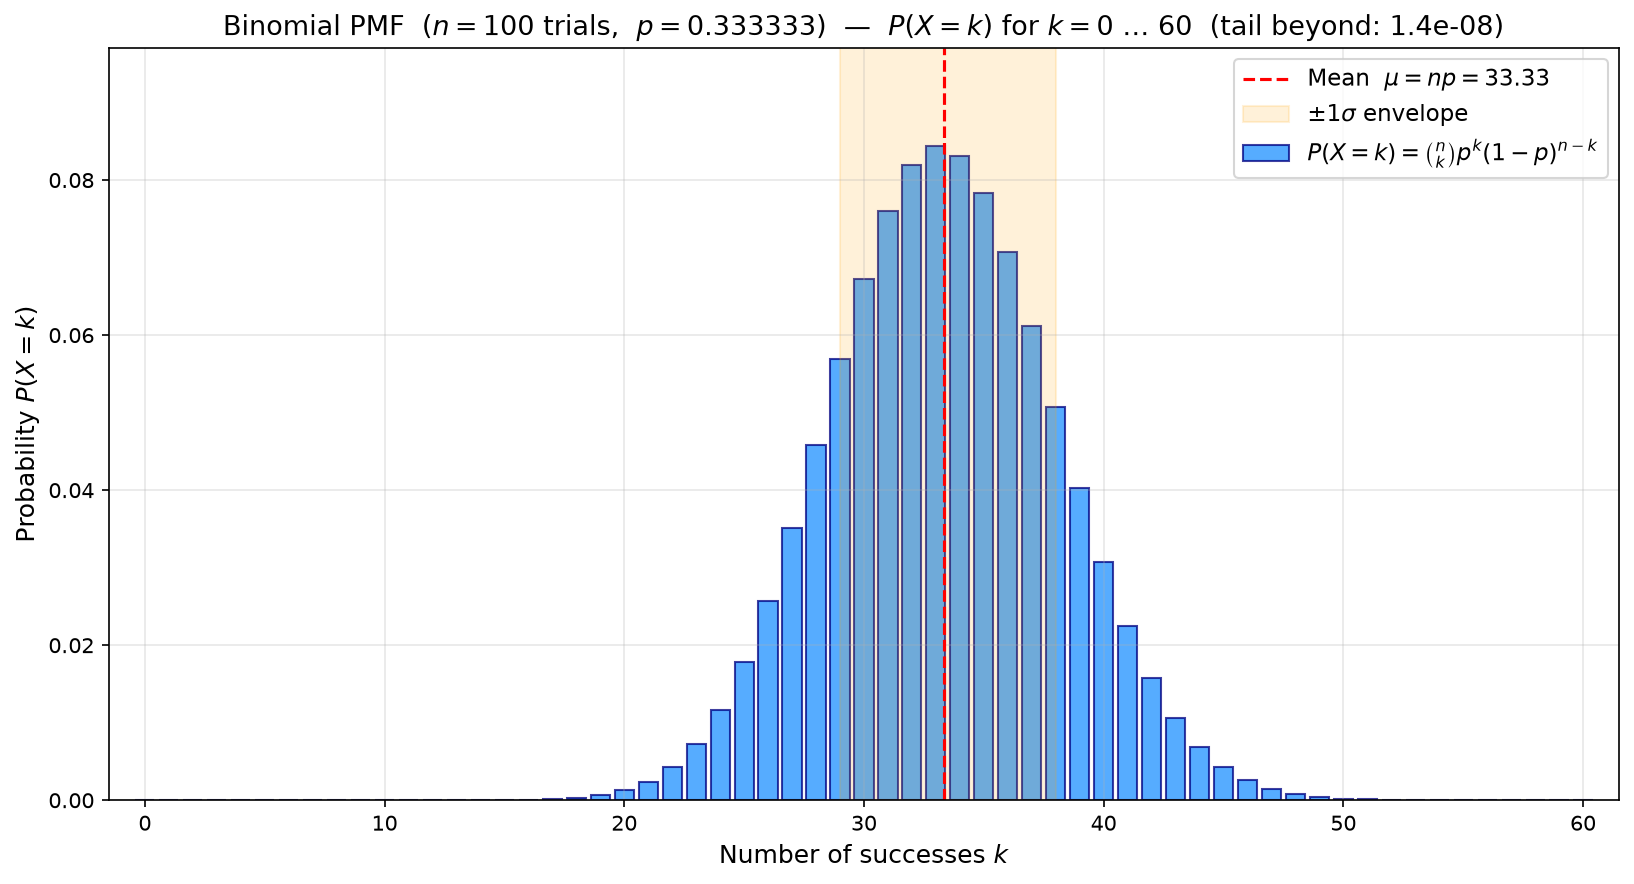
\includegraphics[width=0.9\textwidth]{binomial_pmf_n100_p13.png}
\caption{Función de masa de probabilidad de la distribución binomial con $n=100$ y $p=\frac{1}{3}$: la probabilidad $\PP\{S=k\}=\binom{100}{k}(1/3)^k(2/3)^{100-k}$ para $k=0,\dots,60$, con la media $\mu=np\approx 33.33$.}
\label{fig:binomial_pmf}
\end{figure}


\subsection{Aproximaciones para la distribución binomial}

Esta sección es una tangente del tema central del curso que sirve como motivación para algunas de las ideas que desarrollaremos después. 

La siguiente fórmula provee una aproximación de la densidad binomial $\mu_n(m):=\binom{n}{m}p^mq^{n-m}$ mediante una función muy especial, la llamada \emph{distribución normal o distribución Gaussiana} $\frac{1}{\sqrt{2\pi}}e^{-\frac{x^2}{2}}$ que juega un rol central en probabilidad y  estadística. 

\begin{lemma}Para todo $p\in (0,1)$ y $m=0,\dots, n$, definiendo $x=\frac{m-np}{\sqrt{npq}}$ se tiene que
\[\lim_{n\rightarrow \infty} \frac{\sqrt{npq}\mu_n(m)}{\frac{1}{\sqrt{2\pi}}e^{-\frac{x^2}{2}}}=1\]
\end{lemma}
\noindent
Más precisamente el Lema anterior dice que
\[\mu_n(m)\approx  \frac{1}{\sqrt{2\pi npq}}e^{-\frac{\left(\frac{m-np}{\sqrt{npq}}\right)^2}{2}}\]
provee buenas estimaciones cuando $n>>0$ y $p$ no es ni demasiado grande ni demasiado chico. Esto es muy útil pues el lado derecho es fácilmente aproximable numéricamente.

\begin{figure}[h]
\centering
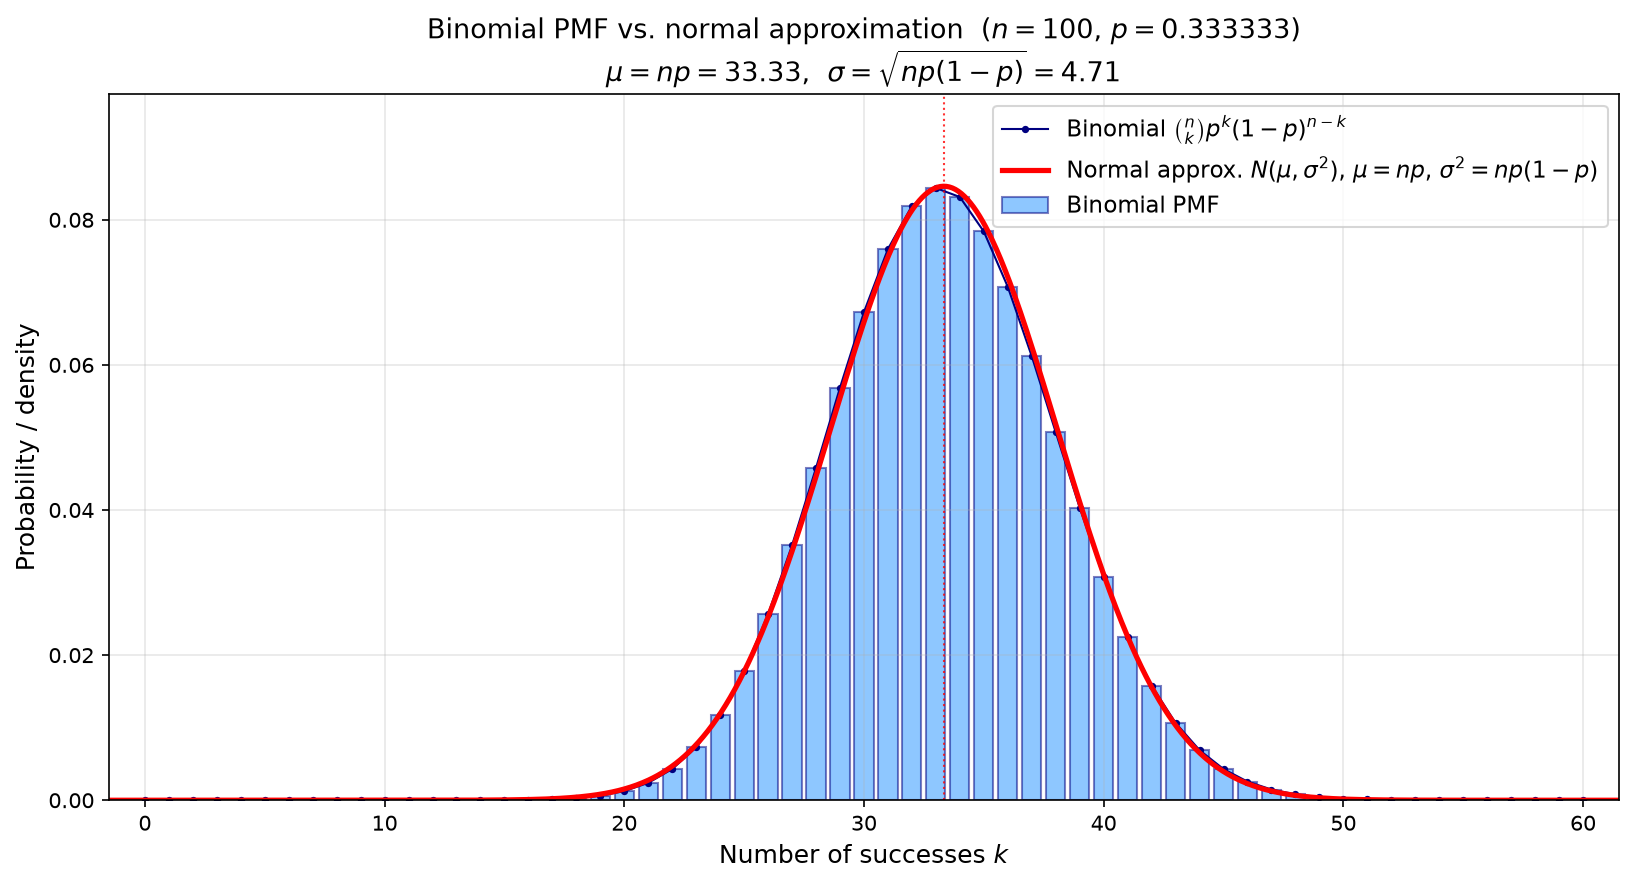
\includegraphics[width=0.9\textwidth]{binomial_pmf_n100_p13_normal.png}
\caption{Función de masa de probabilidad de la distribución binomial con $n=100$ y $p=\frac{1}{3}$ junto con su aproximación normal correspondiente.}
\label{fig:binomial_pmf}
\end{figure}


\subsection{Ejemplo 3: Un espacio de probabilidad continuo}

Queremos construir un modelo probabilista para la siguiente situación: \emph{Se selecciona un número real en el intervalo $[0,1]$ de manera uniforme (de tal forma que todo punto tenga la misma probabilidad)}.

Definimos $\Omega=[0,1]$ definimos $\calF$ como la sigma-\'algebra m\'as pequeña que contiene a los intervalos abiertos $(a,b)\subseteq [0,1]$, esta sigma-álgebra se llama la sigma-álgebra de Borel. Definimos $\PP((a,b)):=b-a$ para cualquier intervalo y más generalmente definimos la probabilidad de cualquier $A\in \calF$ como su longitud (tambien llamada su medida de Lebesgue). Es un hecho (no tan fácil de demostrar y parte de un curso más preciso) que $(\Omega,\calF,\PP)$ es un espacio de probabilidad.

\begin{remark} Bajo este modelo continuo de probabilidad $\PP(\{z\})=0$ para cualquier $z\in [0,1]$. Por lo anterior el comportamiento de la probabilidad debe estudiarse en intervalos. Por ejemplo $\PP([0,z])=z$ para cualquier $z\in [0,1]$ y $\PP([1/3,2/3])=1/3$. 
\end{remark}



\section{Variables aleatorias}
En esta sección introducimos variables aleatorias en $\RR$, sus distribuciones y sus valores esperados. 

\begin{definition} Una \emph{variable aleatoria} $X$ en $(\Omega,\calF,\PP)$ es una función $X:\Omega\rightarrow \RR$ tal que para todos $a,b\in \RR$ el conjunto $\{\omega\in \Omega: a<X(\omega)\leq b\}\in \calF$. La \emph{distribución} de $X$ es la función que mide la probabilidad de que $X$ caiga en cada intervalo $(a,b]$
\[\PP_X\left((a,b]\right):=\PP\left(\left\{\omega\in \Omega: a<X(\omega)\leq b\right\}\right)\]
Para simplificar la notación denotamos
\[\PP\left(\left\{\omega\in \Omega: a<X(\omega)\leq b\right\}\right)=:\PP\left\{a<X\leq b\right\}\]
Típicamente la distribución se resume a través de la \emph{función de distribución acumulada} 
\[F_X(\beta):=\PP\left(\left\{\omega\in \Omega: X(\omega)\leq b\right\}\right)\]
ó usando notación menos recargada $F_X(\beta)=
\PP\{X\leq \beta\}$.
\end{definition}



\begin{examplex} \emph{Lanzamos dos monedas justas $\{0,1\}$ y definimos la variable $X$ como el número de veces que cae $1$.}
Como vimos en la sección anterior,el espacio de probabilidad natural es el modelo de Bernoulli con $p=q=1/2$ y $n=2$. Es decir $\Omega=\{00,01,10,11\}$, $\calF$ son todos los subconjuntos de $\Omega$ y $\PP$ es la distribución uniforme en $\Omega$ (que asigna $1/4$ a cada $\omega\in \Omega$). La función $X$ se puede tabular así:


\begin{center}
\begin{tabular}{c|c}
$\omega$ & $X(\omega)$ \\
\hline
$00$ & $0$ \\
$10$ & $1$ \\
$01$ & $1$ \\
$11$ & $2$
\end{tabular}
\end{center}

De lo anterior vemos que la distribución de $X$ cumple: $X$ cae $0$ con prob $1/4$, cae $1$ con probabilidad $1/2$ (pues es la suma de las probabilidades de las pre-imágenes $01$ y $10$ y cada una contribuye $1/4$) y cae $2$ con probabilidad $1/4$.
\end{examplex}
\begin{examplex} Si en el ejemplo anterior definimos $Y$ como la cantidad de veces que cae cero entonces obtenemos una nueva variable aleatoria distinta de $X$ pues $0=X(00)\neq Y(00)=2$ luego son funciones distintas. No obstante las variables $X$ e $Y$ tienen \emph{la misma distribución}. 
\end{examplex}



\subsection{Distribuciones de probabilidad}

Distinguimos variables aleatorias discretas y continuas. Luego de algunas definiciones preliminares nos ocuparemos del estudio de ejemplos concretos.

\begin{definition} Sea $D\subseteq \RR$ un conjunto discreto.
. Una funci\'on $f_X:D\rightarrow \RR$ es  la densidad de una variable aleatoria discreta $X$ en $D$ si cumple:
\begin{enumerate}
\item $\forall d\in D\left(f_X(d)\geq 0\right)$
\item $\sum_{d\in D} f_X(d)=1$
\end{enumerate}  
La \emph{función de distribución acumulada} de la variable discreta $X$ es la función
\[F(\beta):=\sum_{d\in D: d\leq \beta} f_X(d)\] 
El \emph{valor esperado} de la variable $X$ es el número
\[\EE[X]:=\sum_{d\in D} d f_X(d).\]
\end{definition}


Sea $[a,b]\subseteq \RR$ un intervalo (permitiendo $a=-\infty$ y $b=\infty$).
\begin{definition} Una funci\'on $f_X:[a,b]\rightarrow \RR$ es la densidad de una variable aleatoria absolutamente continua $X$ en $D$ si cumple:
\begin{enumerate}
\item $\forall x\in [a,b]\left(f_X(x)\geq 0\right)$
\item $\int_a^bf_X(x)dx = 1$
\end{enumerate}
La \emph{función de distribución acumulada} de la variable absolutamente continua $X$ es la función
\[F_X(\beta):=\int_a^{\beta} f_X(x)dx\] 
El \emph{valor esperado} de la variable $X$ es el número
\[\EE[X]:=\int_a^b x f_X(x)\]
\end{definition}

Notar que tanto en el caso discreto como el continuo la función $F_X(\beta)=\PP\{X\leq \beta\}$.

\subsection{Ejemplos de variables aleatorias escalares ($1D$)}

En esta subsección ilustramos gráficamente algunas de las distribuciones de probabilidad más comunes para variables aleatorias escalares. En cada figura se marca la media $\EE[X]$ con una línea vertical.

\paragraph{Distribución binomial.} La variable $X\sim \mathrm{Binomial}(n,p)$ tiene masa de probabilidad $\PP\{X=k\}=\binom{n}{k}p^k(1-p)^{n-k}$, media $\EE[X]=np$ y varianza $\mathrm{Var}(X)=np(1-p)$. En la figura se superponen dos casos distintos, $\mathrm{Binomial}(40,\,\frac{1}{4})$ (media $np=10$) y $\mathrm{Binomial}(90,\,\frac{1}{3})$ (media $np=30$), con el fin de apreciar el rango de formas que admite la familia binomial: la media $np$ desplaza la distribución y los parámetros $n$ y $p$ determinan su dispersión (varianza $np(1-p)$).

\begin{figure}[h]
\centering
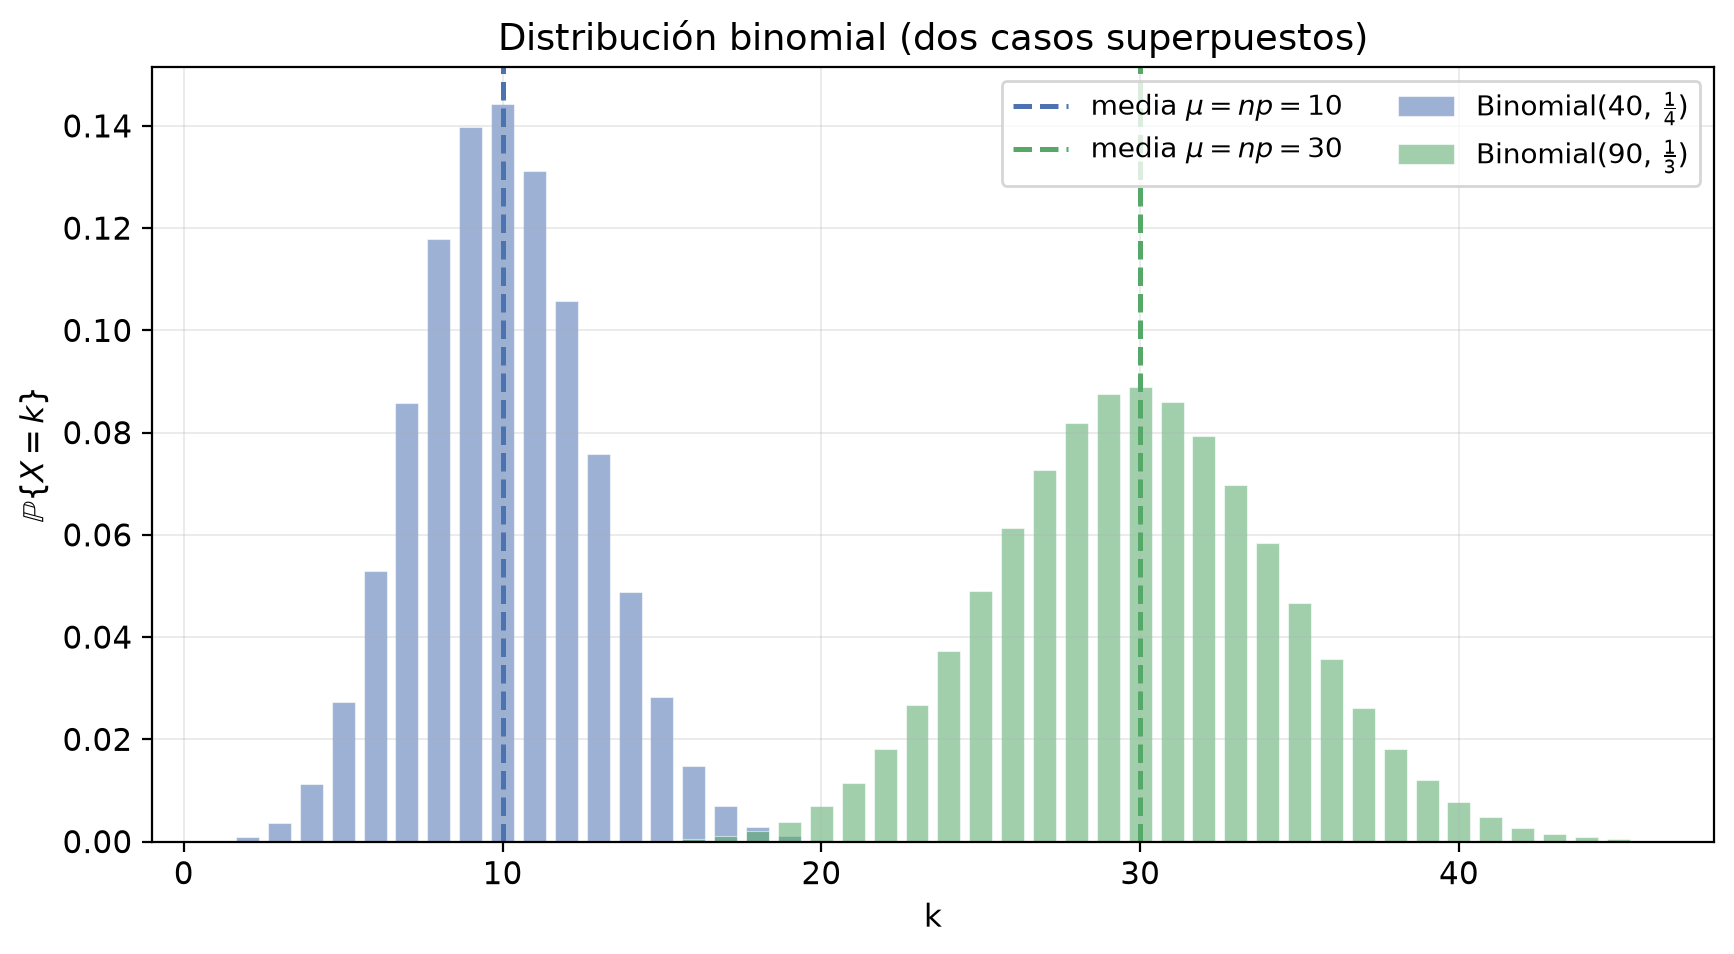
\includegraphics[width=0.9\textwidth]{binomial_pmf.png}
\caption{Función de masa de probabilidad de la distribución binomial, con dos casos superpuestos en el mismo gráfico: $\mathrm{Binomial}(40,\,\frac{1}{4})$ (media $\mu=10$) y $\mathrm{Binomial}(90,\,\frac{1}{3})$ (media $\mu=30$). Las líneas verticales discontinuas (una por cada curva) marcan la media de cada distribución.}
\label{fig:binomial_pmf_example}
\end{figure}

\paragraph{Distribución de Poisson.} La variable $X\sim \mathrm{Poisson}(\lambda)$ tiene masa de probabilidad $\PP\{X=k\}=\frac{\lambda^k e^{-\lambda}}{k!}$, media $\EE[X]=\lambda$ y varianza $\mathrm{Var}(X)=\lambda$. En la figura se superponen los casos $\lambda=10$ y $\lambda=20$, mostrando cómo $\lambda$ desplaza la distribución y, al mismo tiempo, aumenta su dispersión (en Poisson, media y varianza coinciden, ambas iguales a $\lambda$).

\begin{figure}[h]
\centering
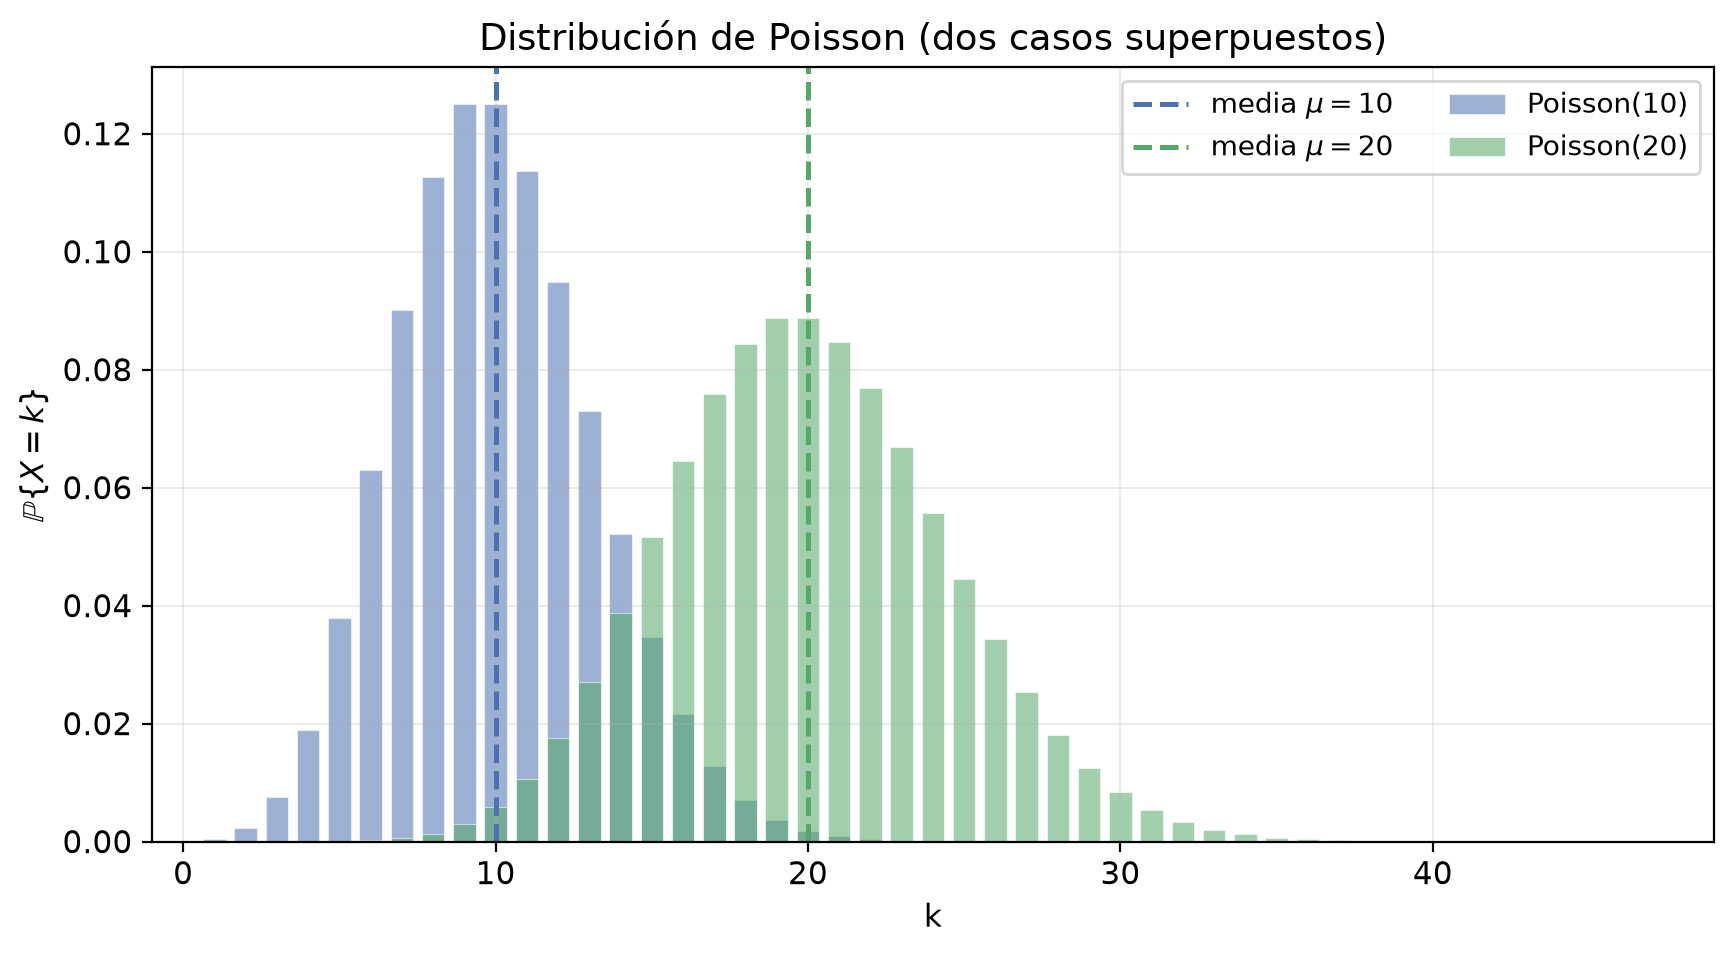
\includegraphics[width=0.9\textwidth]{poisson_pmf.png}
\caption{Función de masa de probabilidad de la distribución de Poisson, con dos casos superpuestos en el mismo gráfico: $\mathrm{Poisson}(10)$ (media $\mu=10$) y $\mathrm{Poisson}(20)$ (media $\mu=20$). Las líneas verticales discontinuas (una por cada curva) marcan la media de cada distribución.}
\label{fig:poisson_pmf_example}
\end{figure}

\paragraph{Distribución gaussiana (normal).} La variable $X\sim \mathrm{Normal}(\mu,\sigma)$ tiene densidad $f_X(x)=\frac{1}{\sigma\sqrt{2\pi}}e^{-\frac{(x-\mu)^2}{2\sigma^2}}$, media $\EE[X]=\mu$ y varianza $\mathrm{Var}(X)=\sigma^2$. En la figura se comparan $\mathrm{Normal}(0,1)$, $\mathrm{Normal}(0,2)$ y $\mathrm{Normal}(3,1)$, observando el efecto de la media y de la desviación estándar.

\begin{figure}[h]
\centering
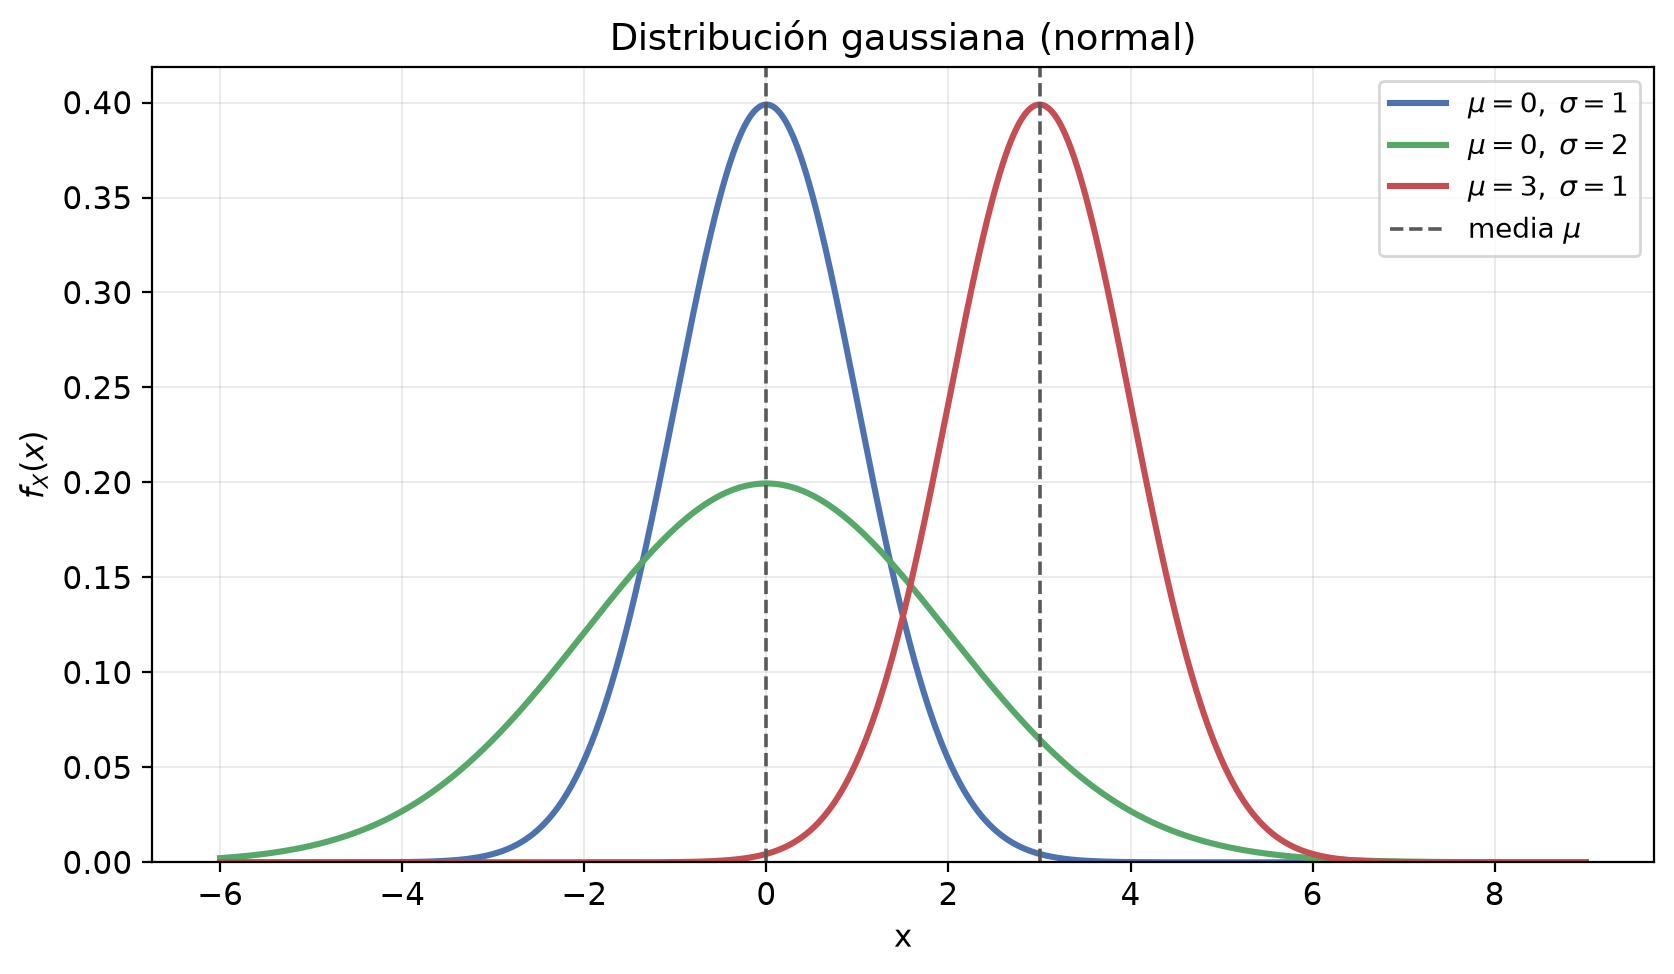
\includegraphics[width=0.9\textwidth]{gaussian_pdf.png}
\caption{Función de densidad de la distribución gaussiana para $\mu=0,\sigma=1$; $\mu=0,\sigma=2$; y $\mu=3,\sigma=1$. Las líneas verticales marcan la media $\mu$ de cada distribución.}
\label{fig:gaussian_pdf_example}
\end{figure}





\end{document}






\begin{enumerate}
\end{enumerate}


\end{enumerate}
\end{enumerate}
\end{definition}

\end{document}

\begin{enumerate}
\item \emph{Fundamentos de Álgebra Lineal:}
\begin{enumerate}
\item \emph{Teorema espectral (en dim finita)}

\begin{theorem}Toda matriz simétrica es ortogonalmente diagonalizable (sobre $\RR$).\end{theorem}
Más generalmente toda matriz normal ($A\in \CC^{n\times n}$ es normal $AA^*=A^*A$) es unitariamente diagonalizable (sobre $\CC$).
\item \emph{Descomposición en valores singulares:}
\begin{theorem} Si $A\in \RR^{m\times n}$ entonces existen matrices ortogonales $U\in \RR^{m\times m}$ y $V\in \RR^{n\times n}$ y una matriz $\Sigma$ diagonal con entradas reales tales que:
\[A=U\Sigma V^T\]
\end{theorem}
M\'as precisamente, podemos asumir que las entradas diagonales no nulas de $\Sigma$ son n\'umeros $\sigma_1\geq \dots \geq  \sigma_r>0$ donde $r={\rm rank}(A)$. Estos números se llaman los {\bf valores singulares} de $A$. 

Observaciones:

\begin{itemize}
\item La demostración de existencia es constructiva (si pudiéramos calcular valores y vectores propios, lo que haremos más adelante) pues se reduce a que:
\begin{enumerate}
\item Las columnas de $U$ pueden ser una base ortonormal de vectores propios de $AA^T$ (con $AA^Tu_i=\sigma_i^2u_i$), extendida a una base ortonormal del espacio completo si el rango lo requiere.
\item Las columnas de $V$ pueden ser una base ortonormal de vectores propios de $A^TA$ (con $A^tAv_i=\sigma_i^2v_i$), extendida a una base ortonormal del espacio completo si el rango lo requiere.
\item Los valores singulares son las raíces de los valores propios no nulos de $AA^T$ \'o $A^TA$. Esto demuestra la unicidad de los valores singulares y tambien explica en qué sentido falla la unicidad de $U$ y $V$.
\end{enumerate}
\item $\Sigma$ es, en general una matrix rectangular del mismo formato que $A$ y sus únicas entradas no nulas estan sobre la diagonal.
\item La descomposición de arriba permite, sumando sobre las entradas diagonales, escribir 
\[A=\sum_{i=1}^r \sigma_i u_iv_i^t\]
expresando $A$ como suma de $r$ matrices de rango uno.
\item Todo lo anterior es válido sobre $\CC$, donde $A\in \CC^{m\times n}$ y las matrices $U$ y $V$ son unitarias, llevando a una descomposición 
\[A=U\Sigma V^*\]
\end{itemize}
\end{enumerate}

\item \emph{Normas:}
\begin{enumerate}
\item Conocer el enunciado de la desigualdad de Holder y poder usarla para demostrar que $\|\bullet\|_p$ es norma en $\RR^n$ para $p\geq 1$. Saber demostrar:

\begin{theorem}
En un espacio vectorial de dimensión finita, todo par de normas son equivalentes.
\end{theorem}


\item \emph{Normas inducidas en espacios de matrices} Definición de la norma inducida sobre operadores $T:V\rightarrow W$ por normas $\|\cdot\|_V$ y $\|\cdot\|_W$ en $V$ y $W$
\[\|T\|_{\rm op}:=\sup_{v\in V\setminus\{0\}} \frac{\|Tv\|_W}{\|v\|_V}.\] 
Saber demostrar que es norma y que cumple $\|Tv\|_W\leq \|T\|_{\rm op}\|v\|_V$. 

\item Saber calcular $\|T\|_{\rm op,1,1}$, $\|T\|_{\rm op,\infty,\infty}$ en términos de las entradas de $T$ y expresar $\|T\|_{\rm op,2,2}$ en términos de valores singulares.  
\end{enumerate}


\item \emph{Números de condición y backward stability:}

\begin{enumerate}
\item Saber la definición formal de {\bf número de condición} y de {\bf número de condición absoluto} en un punto $x\in V$ de una función $f:V\rightarrow W$ entre espacios normados $V$ y $W$ (denotados $k(x,f)$ y $\tilde{k}(x,f)$ respectivamente).

\item Poder demostrar formalmente que el número de condición de {\it resolver el sistema lineal} $Ax=b$ para $b$ fijo esta acotado, para una matriz invertible $A$ por $k(A):=\|A\|\|A^{-1}|$. Si $\|\bullet\|:=\|\bullet\|_{\rm op,2,2}$ poder expresar $k(A)$ en términos de los valores singulares de $A$.

\item Entender la definición de backward-stable:
Para $\epsilon_0>0$ decimos que $\tilde{f}:V\rightarrow W$ es $\epsilon_0$-backward-stable con respecto a $f:V\rightarrow W$ si 
$\forall x\in V \exists \tilde{x}$ que cumple:
\begin{enumerate}
\item $\tilde{f}(x)=f(\tilde{x})$ 
\item $\|x-\tilde{x}\|\leq \epsilon_0\|x\|$
\end{enumerate}

\item Poder demostrar:
\begin{enumerate}
\item  Que una implementación del producto de números $x\ast y$ que garantice 
\[x\ast y = xy(1+\epsilon_0)\]
para todos $x,y$ es $\epsilon_0$-backward stable.
\item Que el producto interno de vectores en $\RR^n$, implementado con operaciones de producto y suma como las anteriores es backward-stable para algún múltiplo explícito de $\epsilon_0$ (para todo $\epsilon_0$ suficientemente pequeño). 

\item \emph{Uso de backward stability:}
\begin{theorem} Si $\tilde{f}$ es una implementación $\epsilon_0$-backward stable de $f$ entonces el error relativo en $x$ esta controlado por el número de condición $K(x,f)$  de $f$ en $x$. Más precisamente, si $f(x)\neq 0$ tenemos la siguiente desigualdad
\[\frac{\|\tilde{f}(x)-f(x)\|}{\|f(x)\|}\leq K(x,f)\epsilon_0\]
\end{theorem}

\item \begin{theorem} Resolver un sistema lineal triangular inferior mediante sustitución hacia atrás es backward-stable.
\end{theorem} 
Saber la demostración para sistemas $2\times 2$ (la idea en general es la misma y solo requiere más cálculos)

\end{enumerate}


\end{enumerate}
\item \emph{Factorización LU}:
\begin{enumerate}
\item Saber qué es la factorización $LU$ de una matriz cuadrada $A$.
\item Cómo usarías una factorización $A=LU$ conocida para resolver el sistema $Ax=b$? Qué puedes decir del número de condición y del error relativo de ese algoritmo?
\item Demostrar que si $A$ es invertible y la factorización $LU$ existe entonces es única. Existe siempre tal factorización? De existir es siempre única (removiendo el requisito de invertibilidad de $A$)?

\item Calcular la factorización $LU$ de la matriz 
$\begin{pmatrix}
\epsilon & 1 \\
1 & 1
\end{pmatrix}$
para $\epsilon\neq 0$. Notar la descomposición $LU$ no existe cuando $\epsilon=0$. Qué pasa con los números de condición de los factores $L$ y $U$ cuando $\epsilon\rightarrow 0$?


\item \emph{Criterio de existencia útil, sin pivoteo y consecuencias en matrices simétricas} Sea $A\in \RR^{n\times n}$ una matriz y sea $A_{\leq p}$ la submatriz cuadrada con índices de filas y columnas $\leq p$.

\begin{theorem} Si $\det(A_p)\neq 0$ para todo $p$ entonces existe una matriz triangular inferior con diagonal de $1$'s $L$ y una matriz triangular superior $U$ tal que $A=LU$.
\end{theorem}

\begin{theorem} [Sylvester + factorización de Cholesky] Si $A$ es simétrica y $\det(A_p)>0$ para todo $p$ entonces existe una única matriz invertible, triangular inferior $C$ con entradas positivas en la diagonal que cumple $A=CC^T$.
\end{theorem}

Más generalmente, si $\det(A_p)\neq 0$ para todo $p$ y $A$ es simétrica entonces existe una descomposición $A=LDL^T$ donde $L$ es triangular inferior con diagonal de unos y $D$ es una matriz diagonal.

\item Saber que, por Gauss-Jordan, TODA matriz admite una descomposición $LU$ con pivoteo $PA=LU$ para alguna permutación $P$. \emph{Dato curioso (sin dem.)} para TODA matriz simétrica $A$ existe una permutación $P$ tal que $P^T A P = LDL^T$ donde $L$ es triangular inferior con unos en la diagonal, $D$ es diagonal \emph{por bloques} donde todos los bloques tienen tamaño $2\times 2$ ó $1\times 1$). Ejemplo: $\begin{pmatrix}
0 & 1 \\
1 & 0
\end{pmatrix}$ necesita bloques $2\times 2$.
\end{enumerate}

\item {\it Factorización QR}:
\begin{enumerate}

\item \begin{theorem} Una matriz $Q\in \RR^{n\times n}$ es \emph{ortogonal} si satisface cualquiera de las siguientes propiedades equivalentes:
\begin{enumerate}
\item $\|Qx\|_2=\|x\|_2$ para todo $x\in \RR^n$.
\item $\langle Qx,Qy\rangle = \langle x,y\rangle $ para todos $x,y\in \RR^n$.
\item $QQ^T=Id$ (ó equivalentemente $Q^TQ=I$). 
\end{enumerate}
\end{theorem}

\item La {\bf reflexión de Householder} ortogonal al vector unitario $w\in \RR^n$ es la transformación
\[H_w(x)=x-2\frac{\langle w,x\rangle}{\langle w,w\rangle} w\]
Definimos $H_0(x):=x$. Saber demostrar sus propiedades principales, resumidas en el siguiente Lema,
\begin{lemma} Las siguientes propiedades son ciertas si $w\neq 0$,
\begin{enumerate}
\item $H_w$ es la reflexión respecto al hiperplano perpendicular a $w$.
\item $H_w$ es simétrica, ortogonal y $\det(H_w)=-1$.
\item Para todo vector $a\in \RR^n$ existe un vector unitario $w$ ó $w=0$ tal que $H_w(a)=\|a\|e_1$ donde $e_1=(1,0,\dots,0)$ es el primer vector de la base canónica.
\end{enumerate}
\end{lemma}


\item Conocer la demostración del siguiente Teorema, usando reflexiones de Householder
\begin{theorem} Para toda matriz $A\in \RR^{m\times n}$ con $m\geq n$ existe una matriz ortogonal $Q$ y una matriz triangular superior $R$ tal que $A=QR$.
\end{theorem}

\item Saber explicar formalmente la frase {\it existe una implementación backward-stable de la factorización $QR$}.

\item Poder demostrar que el número de condición de $A$ es igual al número de condición de $R$ si $A=QR$. Cómo se podría usar la factorización $QR$ para resolver el sistema lineal $Ax=b$ cuando $A$ es invertible y qué tipo de garantías sobre el error podemos demostrar?

\item Suponga que $A\in \RR^{m\times n}$ con $m\leq n$. Poder explicar cómo puede usarse la factorización de $QR$ de la matriz $A$ para resolver el problema de regresión lineal
\[\min_{x\in \RR^n} \|Ax-b\|_2^2\]
reduciéndolo a resolver cierto sistema lineal triangular. Qué sucede si ${\rm rank}(A)<n$?

\end{enumerate}


\end{enumerate}

\end{document}
